\documentclass[letterpaper,10pt]{article}
\usepackage[utf8]{inputenc}
\usepackage[activeacute,spanish]{babel}
\usepackage{amsmath}
\usepackage{amsfonts}
\usepackage{enumerate}
\usepackage{float}
\usepackage{indentfirst}
\usepackage{graphicx}
\usepackage{url}
\usepackage{multicol}
\usepackage{subfigure}
\usepackage[position=bottom]{subfig}
\usepackage{geometry}
\usepackage{fullpage}
\usepackage{algorithmic}
\usepackage{algorithm}

\setlength\parindent{0pt}

\usepackage{tikz}
\usetikzlibrary{arrows,petri,topaths,shapes,automata}

\tikzset{
    %Define standard arrow tip
    >=stealth',
    % Define arrow style
    pil/.style={
           ->,
           thick,}
}

\begin{document}

\thispagestyle{empty}

\begin{minipage}[t]{0.6\textwidth}
{\Large \textbf{INF152} Estructuras Discretas}

{\large Profesores: C. Lobos -- M. Bugueño -- S. Gallardo}

Universidad Técnica Federico Santa María

Departamento de Inform\'atica -- Mayo 14, 2021.

\end{minipage}
\hfill
\begin{minipage}[t]{0.35\textwidth}
%RELLENE CON SUS DATOS PERSONALES:
\textbf{Nombre}: Bryan González\\[0.3cm]
\textbf{Rol}: 202073500-0 \textbf{Paralelo}: 0
\end{minipage}

\vspace{0cm}

\begin{center}
    {\Large Tarea 2} \\ Fecha de entrega Miércoles \textbf{26 de Mayo 23:59}
\end{center}

%%%%%%%%%%%%%%%%%% Fin Header
\hrule 
\vspace{0.2cm}
Esta actividad tiene como objetivo el que usted continúe su aprendizaje en torno a \LaTeX{} demostrando sus habilidades para la creación y manipulación de grafos y \texttt{algoritmos}. Para la entrega digital, cree una carpeta de nombre Actividad2-Latex-rol, y dentro de ella, incluya su archivo .tex y todo lo nencesario para compilar. A partir de la carpeta, cree un archivo comprimido titulado Actividad2-Latex-rol y súbalo a Aula en la sección correspondiente.

\vspace{0.2cm}
\hrule 

\vspace{0.4cm} 

\begin{minipage}{0.65\linewidth}
El paquete Tikz es probablemente la herramienta más compleja y poderosa para crear elementos gráficos en \LaTeX. A lo largo de este curso, este paquete será su salvador cuando de grafos se trate. Tikz nos permite aplicar una gran variedad de líneas, curvas, colores, figuras, entro otras muchas características, algunas de las cuales se muestran en la Figura \ref{muestra}.
\end{minipage}
\hfill
\begin{minipage}{0.32\linewidth}
          \centering
            \begin{tikzpicture}[scale=1,transform shape,node distance=2.5cm,main node/.style={circle,draw}]
		    %nodes
			\node[main node] (1) 			{$A$};
			\node[main node] (2) [right of=1] 	    {$B$};
		    %Edges
			\path (1) edge [post, bend left,-] node [above left] {3} (2);
        \end{tikzpicture}
        \captionof{figure}{Ejemplo Tikz.}
        \label{muestra}
\end{minipage}

\vspace{0.4cm}

Utilizando las herramientas que proporciona el paquete, complete los siguientes desafíos:
\begin{enumerate}[1)]
\item Metro de Santiago ha crecido bastante a lo largo de los últimos años. Como puede notar, esta gran red podemos representarla como un grafo donde los nodos corresponderían a las estaciones de metro, mientras que los arcos corresponderían a las vías que interconectan estaciones. La Figura \ref{fig:metro} muestra 19 estaciones, algunas de las cuales corresponden a \textbf{estaciones comunes} pues interconectan dos o más \textbf{líneas de metro}. \\
Utilizando Tikz, se le solicita dibujar un grafo que represente la sección de red de Metro de la Figura \ref{fig:metro}, sujeto a las siguientes restricciones: 
\begin{itemize}
    \item Ser fiel al tipo de arco utilizado en la figura. Esto es, usar aristas arqueadas o rectas cuando así se requiera.
    \item Todas las aristas que formen parte de la Línea 1 (en rojo en Figura \ref{fig:metro}), deberán ser \textbf{líneas segmentadas}.
    \item Toda estación común deberá ser representada utilizando un nodo de forma cuadrada. 
    \item Junto a cada nodo (no dentro), indicar el nombre de la estación de metro.
\end{itemize} 

\begin{minipage}{\linewidth}
      \centering
      \begin{minipage}{0.8\linewidth}
          \begin{figure}[H]
              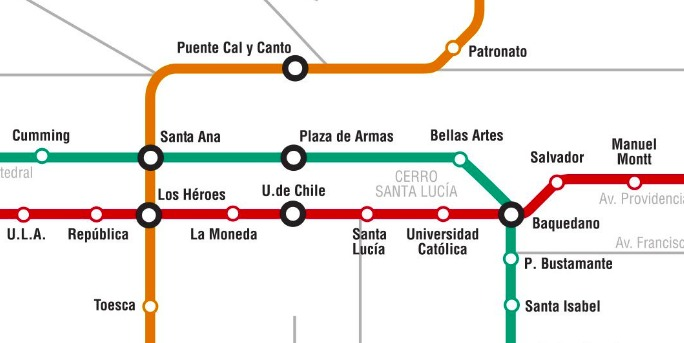
\includegraphics[width=0.9\linewidth]{sec_metro.jpeg}
              \caption{Sección Metro de Santiago, 2010}
              \label{fig:metro}
          \end{figure}
      \end{minipage}
  \end{minipage}

\begin{center}
    \tikzstyle{normal}=[circle,draw=black,very thick,inner sep=2pt]
    \tikzstyle{importante}=[circle,draw=black,ultra thick,inner sep=3pt]
    \tikzstyle{comun}=[rectangle,draw=black,very thick,inner sep=4pt]
    \tikzstyle{every label}=[scale=0.2mm,align=center]
    \resizebox{15cm}{6cm}{
    \begin{tikzpicture}[ultra thick]
        \node[normal] (patronato) at (2.5,2) [label=right:\textbf{Patronato}] {};
        \node[importante] (puente_cal_y_canto) at (0,1.7) [label=above left:\textbf{Puente Cal y Canto}] {};
        \node[comun] (santa_ana) at (-2.5,0.2) [label=above right:\textbf{Santa Ana}] {};
        \node[importante] (plaza_de_armas) at (0,0.2) [label={[label distance=0.1mm]80:\textbf{Plaza de Armas}}] {};
        \node[normal] (bellas_artes) at (2.6,0.2)  [label=above :\textbf{Bellas Artes}]  {};
        \node[normal] (cumming) at (-4.5,0.2)  [label=above:\textbf{Cumming}] {};
        \node[importante] (u_de_chile) at (0,-0.8)  [label=above:\textbf{U. de Chile}] {};
        \node[normal] (la_moneda) at (-1.2,-0.8)  [label=below:\textbf{La Moneda}] {};
        \node[normal] (santa_lucia) at (1.2,-0.8) [label=below:\textbf{Santa}\\\textbf{Lucía}] {};
        \node[normal] (universidad_catolica) at (2.3,-0.8) [label=below:\textbf{Universidad}\\\textbf{Católica}] {};
        \node[comun] (baquedano) at (3.5,-0.8) [label={[label distance=0.1mm]-15:\textbf{Baquedano}}] {};
        \node[normal] (p_bustamante) at (3.5,-1.5) [label=right:\textbf{P. Bustamante}] {};
        \node[normal] (santa_isabel) at (3.5,-2.2) [label=right:\textbf{Santa Isabel}] {};
        \node[normal] (salvador) at (4.3,-0.2) [label=above:\textbf{Salvador}] {};
        \node[normal] (manuel_montt) at (5.4,-0.2) [label=above:\textbf{Manuel}\\\textbf{Montt}]  {};
        \node[comun] (los_heroes) at (-2.5,-0.8) [label={[label distance=0.1mm]85:\textbf{Los Héroes}}] {};
        \node[normal] (republica) at (-3.4,-0.8) [label=below:\textbf{República}] {};
        \node[normal] (ula) at (-4.8,-0.8) [label=below:\textbf{U.L.A}] {};
        \node[normal] (toesca) at (-2.5,-2.2) [label=left:\textbf{Toesca}] {};
        \draw (santa_ana) --(plaza_de_armas);
        \draw (santa_ana) --(cumming);
        \draw (santa_ana) --(los_heroes);
        \draw (plaza_de_armas) --(bellas_artes);
        \draw (bellas_artes) --(baquedano);
        \draw (baquedano) --(p_bustamante);
        \draw (p_bustamante) --(santa_isabel);
        \draw (los_heroes) --(toesca);
        \draw[dashed] (ula) -- (republica);
        \draw[dashed] (republica) -- (los_heroes);
        \draw[dashed] (los_heroes) -- (la_moneda);
        \draw[dashed] (la_moneda) -- (u_de_chile);
        \draw[dashed] (u_de_chile) -- (santa_lucia);
        \draw[dashed] (santa_lucia) -- (universidad_catolica);
        \draw[dashed] (universidad_catolica) -- (baquedano);
        \draw[dashed] (baquedano) -- (salvador);
        \draw[dashed] (salvador) -- (manuel_montt);
        \draw[rounded corners=5mm] (puente_cal_y_canto)-- (-2.5,1.7) -- (santa_ana);
        \draw[rounded corners=1mm] (patronato)-- (2.2,1.7) -- (puente_cal_y_canto);
\end{tikzpicture}
    }
\end{center}



\item ¡Subamos la complejidad! Utilizando Tikz, agregue el color correspondiente a cada nodo y arco del grafo construido en el ítem anterior. \textbf{Para estaciones comunes utilice \textbf{negro}}. Además, en al menos 3 arcos, indique la distancia en kilómetro que existe entre las estaciones en cuestión (una distancia arbitraria, no es necesario investigar sobre el asunto).

\begin{center}
    \tikzstyle{normal}=[circle,draw=black,very thick,inner sep=2pt]
    \tikzstyle{importante}=[circle,draw=black,ultra thick,inner sep=3pt]
    \tikzstyle{comun}=[rectangle,draw=black,very thick,inner sep=4pt]
    \tikzstyle{every label}=[scale=0.2mm,align=center]
    \resizebox{15cm}{6cm}{
    \begin{tikzpicture}[ultra thick]
        \node[normal,orange] (patronato) at (2.5,2) [label=right:\textbf{Patronato}] {};
        \node[importante,orange] (puente_cal_y_canto) at (0,1.7) [label=above left:\textbf{Puente Cal y Canto}] {};
        \node[comun] (santa_ana) at (-2.5,0.2) [label=above right:\textbf{Santa Ana}] {};
        \node[importante,green!70!blue!60!black] (plaza_de_armas) at (0,0.2) [label={[label distance=0.1mm]80:\textbf{Plaza de Armas}}] {};
        \node[normal,green!70!blue!60!black] (bellas_artes) at (2.6,0.2)  [label=above :\textbf{Bellas Artes}]  {};
        \node[normal,green!70!blue!60!black] (cumming) at (-4.5,0.2)  [label=above:\textbf{Cumming}] {};
        \node[importante,red] (u_de_chile) at (0,-0.8)  [label=above:\textbf{U. de Chile}] {};
        \node[normal,red] (la_moneda) at (-1.2,-0.8)  [label=below:\textbf{La Moneda}] {};
        \node[normal,red] (santa_lucia) at (1.2,-0.8) [label=below:\textbf{Santa}\\\textbf{Lucía}] {};
        \node[normal,red] (universidad_catolica) at (2.3,-0.8) [label=below:\textbf{Universidad}\\\textbf{Católica}] {};
        \node[comun] (baquedano) at (3.5,-0.8) [label={[label distance=0.1mm]-15:\textbf{Baquedano}}] {};
        \node[normal,green!70!blue!60!black] (p_bustamante) at (3.5,-1.5) [label=right:\textbf{P. Bustamante}] {};
        \node[normal,green!70!blue!60!black] (santa_isabel) at (3.5,-2.2) [label=right:\textbf{Santa Isabel}] {};
        \node[normal,red] (salvador) at (4.3,-0.2) [label=above:\textbf{Salvador}] {};
        \node[normal,red] (manuel_montt) at (5.4,-0.2) [label=above:\textbf{Manuel}\\\textbf{Montt}]  {};
        \node[comun] (los_heroes) at (-2.5,-0.8) [label={[label distance=0.1mm]85:\textbf{Los Héroes}}] {};
        \node[normal,red] (republica) at (-3.4,-0.8) [label=below:\textbf{República}] {};
        \node[normal,red] (ula) at (-4.8,-0.8) [label=below:\textbf{U.L.A}] {};
        \node[normal,orange] (toesca) at (-2.5,-2.2) [label=left:\textbf{Toesca}] {};
        \draw[green!70!blue!60!black] (santa_ana) --(plaza_de_armas)
        node[midway,below,black,scale=0.25mm] {3[km]};
        \draw[green!70!blue!60!black] (santa_ana) --(cumming);
        \draw[orange] (santa_ana) --(los_heroes);
        \draw[green!70!blue!60!black] (plaza_de_armas) --(bellas_artes)
        node[midway,below,black,scale=0.25mm] {5[km]};
        \draw[green!70!blue!60!black] (bellas_artes) --(baquedano);
        \draw[green!70!blue!60!black] (baquedano) --(p_bustamante);
        \draw[green!70!blue!60!black] (p_bustamante) --(santa_isabel);
        \draw[orange] (los_heroes) --(toesca)
        node[midway,right,black,scale=0.25mm] {1.5[km]};
        \draw[dashed,red] (ula) -- (republica);
        \draw[dashed,red] (republica) -- (los_heroes);
        \draw[dashed,red] (los_heroes) -- (la_moneda);
        \draw[dashed,red] (la_moneda) -- (u_de_chile);
        \draw[dashed,red] (u_de_chile) -- (santa_lucia);
        \draw[dashed,red] (santa_lucia) -- (universidad_catolica);
        \draw[dashed,red] (universidad_catolica) -- (baquedano);
        \draw[dashed,red] (baquedano) -- (salvador);
        \draw[dashed,red] (salvador) -- (manuel_montt);
        \draw[rounded corners=5mm,orange] (puente_cal_y_canto)-- (-2.5,1.7) -- (santa_ana);
        \draw[rounded corners=1mm,orange] (patronato)-- (2.2,1.7) -- (puente_cal_y_canto);
\end{tikzpicture}
    }
\end{center}

\item Tikz no solo nos apoyará en la construcción de grafos, sino que podremos escribir algoritmos a través de pseudo--códigos. Un ejemplo (sin sentido) se muestra en el Algoritmo \ref{alg:pri}.

\begin{minipage}{0.4\textwidth}
\begin{algorithm}[H]
\begin{algorithmic}[1]
\STATE{\textbf{procedure} nombre(\(G\))}
\STATE{\(Set<Graph> L\)}
\WHILE{\(len(R) \neq len(V)\)}
	\STATE{\(v = (V-R).pop()\)}
\ENDWHILE
\RETURN{\(L\)}
\end{algorithmic}
\caption{Mi algoritmo}
\label{alg:pri}
\end{algorithm}
\end{minipage}
\hfill
\begin{minipage}{0.55\textwidth}
Escriba dos algoritmos cualquiera (sin sentido si quie-\\re) que contengan: \texttt{for, foreach, while, if, else,\\ return}, instrucciones para asignar valores a variables y operaciones.
\textbf{¡Importante!} Es imperativo que uno de sus algoritmos llame al otro en alguna línea. 
\end{minipage}
\end{enumerate}
\begin{center}
    \begin{minipage}{0.5\textwidth}
        \begin{algorithm}[H]
            \begin{algorithmic}[1]
            \STATE{\(string\: Nombre= "Bryan"\);}
            \STATE{ \(int\:j=0\);}
            \FOR{\((int \:i=0;i<Nombre.length();i++)\)}
                \STATE{\(j+=1\);}
            \ENDFOR
            \WHILE{\(j>0\)}
                \IF{$j>5$}
                    \STATE{\(j+=10\);}
                \ELSE
                    \STATE{\(j-=1\);}
                \ENDIF
            \ENDWHILE
            \STATE{\(a=[1,2,3]\);}
            \STATE{a.\textbf{foreach(}$j+=a[index]$\textbf{)}; }
            \RETURN{\(j\)}
            \end{algorithmic}
            \caption{Alg1}
            \label{alg:sec}
        \end{algorithm}
        
    \end{minipage}
\end{center}
\begin{center}
    \begin{minipage}{0.5\textwidth}
        \begin{algorithm}[H]
            \begin{algorithmic}[1]
            \STATE{\(int\: c = 5\);}
            \IF{$c=5$}
                \STATE{$x =$\textbf{Alg1()}}
            \ELSE
                \STATE{\(int\:j = 1\);}
            \ENDIF
            \STATE{\(num=[1,2,3]\);}
            \FOR{\((int \:i=0;i<num.length();i++)\)}
                \STATE{\(c+=1\);}
            \ENDFOR
            \WHILE{\(c>0\)}
                \STATE{$T=[3,2,1]$}
                \STATE{\(c-=1\)}
            \ENDWHILE
            \STATE{a.\textbf{foreach(}$c+=T[index]$\textbf{)}; }
            \RETURN{\(c\)}
            \end{algorithmic}
            \caption{Alg2}
            \label{alg:tri}
        \end{algorithm}
        
    \end{minipage}
\end{center}


%RECUERDE PONER NOMBRE, ROL Y PARALELO EN EL ENCABEZADO

%NO borre lo que sigue porque no compilará
\end{document}


